% !TEX program = xelatex
\documentclass[12pt,a4paper]{article}

% =================== PACKAGES ===================
\usepackage[T1]{fontenc}
\usepackage{geometry}
\usepackage{graphicx}
\usepackage{hyperref}
\usepackage{enumitem}
\usepackage{titlesec}
\usepackage{fancyhdr}
\usepackage{booktabs}
\usepackage{array}
\usepackage{tabularx}
\usepackage{setspace}
\usepackage[final,nopatch=footnote]{microtype}
\usepackage{newtxtext}
\usepackage{parskip}
\usepackage[nottoc]{tocbibind}
\usepackage{tikz}
\usetikzlibrary{arrows.meta, positioning, shapes.geometric, backgrounds, calc, fit, matrix}
\usepackage{caption}
\captionsetup{font=small, labelfont=bf, margin=0.5cm}
\usepackage{float}
\usepackage{xcolor}
\usepackage{pdflscape}
\usepackage{ragged2e}
\graphicspath{{/Users/krust/Documents/eaClass/Seminar4/}}

% =================== PAGE LAYOUT ===================
\geometry{
  top=1in,
  bottom=1in,
  left=1.05in,
  right=1.05in,
  headheight=14pt,
  headsep=18pt
}
\setstretch{1.12}
\setlength{\emergencystretch}{2em}

% =================== COLOURS ===================
\definecolor{lkblue}{HTML}{1F5B8F}
\definecolor{lkcyan}{HTML}{E9F4FB}
\definecolor{lkgreen}{HTML}{2E7D32}
\definecolor{lkorange}{HTML}{C46A1A}
\definecolor{lkpurple}{HTML}{6A4C93}
\definecolor{lkgray}{HTML}{F4F6F8}
\definecolor{darkgray}{HTML}{333333}
\definecolor{modelyellow}{HTML}{FFF4A3}
\definecolor{modelborder}{HTML}{2B2B2B}

% =================== HEADER / FOOTER ===================
\pagestyle{fancy}
\fancyhf{}
\fancyhead[L]{\small IK2015 Enterprise Architecture}
\fancyhead[R]{\small Seminar 4: Conceptual Model}
\fancyfoot[C]{\thepage}
\renewcommand{\headrulewidth}{0.4pt}

% =================== SECTION FORMATTING ===================
\titleformat{\section}[hang]{\Large\bfseries\color{darkgray}}{\thesection}{1em}{}
\titleformat{\subsection}[hang]{\large\bfseries\color{darkgray}}{\thesubsection}{1em}{}
\titleformat{\subsubsection}[hang]{\normalsize\bfseries\color{darkgray}}{\thesubsubsection}{1em}{}
\titlespacing*{\section}{0pt}{12pt}{6pt}
\titlespacing*{\subsection}{0pt}{10pt}{4pt}
\titlespacing*{\subsubsection}{0pt}{8pt}{2pt}

% =================== HYPERLINK SETUP ===================
\hypersetup{
  colorlinks=true,
  linkcolor=black,
  citecolor=black,
  urlcolor=lkblue,
  pageanchor=false
}

% =================== TABLE HELPERS ===================
\newcolumntype{Y}{>{\RaggedRight\arraybackslash}X}
\newcolumntype{P}[1]{>{\RaggedRight\arraybackslash}p{#1}}
\renewcommand{\arraystretch}{1.28}
\newcommand{\portraitlandscapepagenumber}{%
  \begin{tikzpicture}[remember picture,overlay]
    \node[rotate=90] at ($(current page.east)+(-0.22in,0)$) {\thepage};
  \end{tikzpicture}%
}

% =================== MODEL MACROS ===================
\newcommand{\modelitem}[1]{\item \scriptsize #1}
\newcommand{\roleitem}[2]{\item \scriptsize \textcolor{#1}{#2}}

% =================== TITLE AREA ===================
\title{}
\author{}
\date{}

\begin{document}

% ---- Custom Title Page ----
\thispagestyle{empty}
\vspace*{1.8cm}

\begin{center}
  {\normalsize Jiangxi University of Finance and Economics} \\[2.1cm]

  {\LARGE\bfseries Conceptual Model Report} \\[1.0cm]

  {\Large Luckin Coffee Inc.} \\[0.25cm]
  {\normalsize\itshape A Technology-Driven New Retail Coffee Enterprise} \\[2.0cm]

  {\normalsize IK2015: Enterprise Architecture and Database Programming} \\[0.2cm]
  {\normalsize Seminar 4} \\[2.2cm]

  {\normalsize\textbf{Group 4}} \\[0.45cm]
  {\normalsize
    Zhe-Kai Yang~(Krust),\quad
    Shi-Hang Chen~(Sean),\quad
    Wei-Yu Cai~(Nosta), \\[0.2cm]
    Huan-Wen Chen~(Evan),\quad
    Yuan-Yong Liao~(Foreve)
  } \\[1.8cm]

  {\normalsize \today}
\end{center}

\newpage
\hypersetup{pageanchor=true}
\setcounter{page}{1}
\pagenumbering{arabic}
\pagestyle{fancy}

% =================== BASIC INFORMATION ===================
\section{Report Basic Information}

\begin{table}[H]
\centering
\caption{Basic information of the conceptual modelling report.}
\begin{tabularx}{\textwidth}{P{4.2cm}Y}
\toprule
\textbf{Item} & \textbf{Information} \\
\midrule
Selected enterprise / business & Luckin Coffee Inc.; mobile-first coffee retail, pickup, delivery, partnership-store operation, and packaged coffee business. \\
Course and seminar & IK2015 Enterprise Architecture and Database Programming; Seminar 4. \\
Group number & Group 4. \\
Group members & \parbox[t]{\hsize}{\raggedright Zhe-Kai Yang~(Krust), Shi-Hang Chen~(Sean), Wei-Yu Cai~(Nosta),\\ Huan-Wen Chen~(Evan), Yuan-Yong Liao~(Foreve).} \\
Main deliverable & A conceptual model for the Luckin Coffee case study and a written explanation of its objects, relationships, attributes, and business meaning. \\
\bottomrule
\end{tabularx}
\end{table}

The report develops a conceptual model for Luckin Coffee by identifying the key business objects, their relationships, and the variables needed for measurement and decision-making. This is appropriate for Luckin because its business operates as a digital-to-physical retail system: customers order through mobile channels, stores fulfil orders, delivery partners support logistics, and management systems monitor revenue, quality, inventory, and customer behaviour.

% =================== MODELLING SCOPE ===================
\section{Modelling Scope and Design Logic}

The conceptual model focuses on Luckin Coffee's daily operating logic, from customer demand to order fulfilment and performance feedback. It covers six domains: customer and membership management, digital ordering, store fulfilment, product and recipe management, supply-chain resources, and performance analytics. These domains directly support Luckin's value proposition of convenient, affordable, and reliable coffee consumption.

\begin{figure}[H]
  \centering
  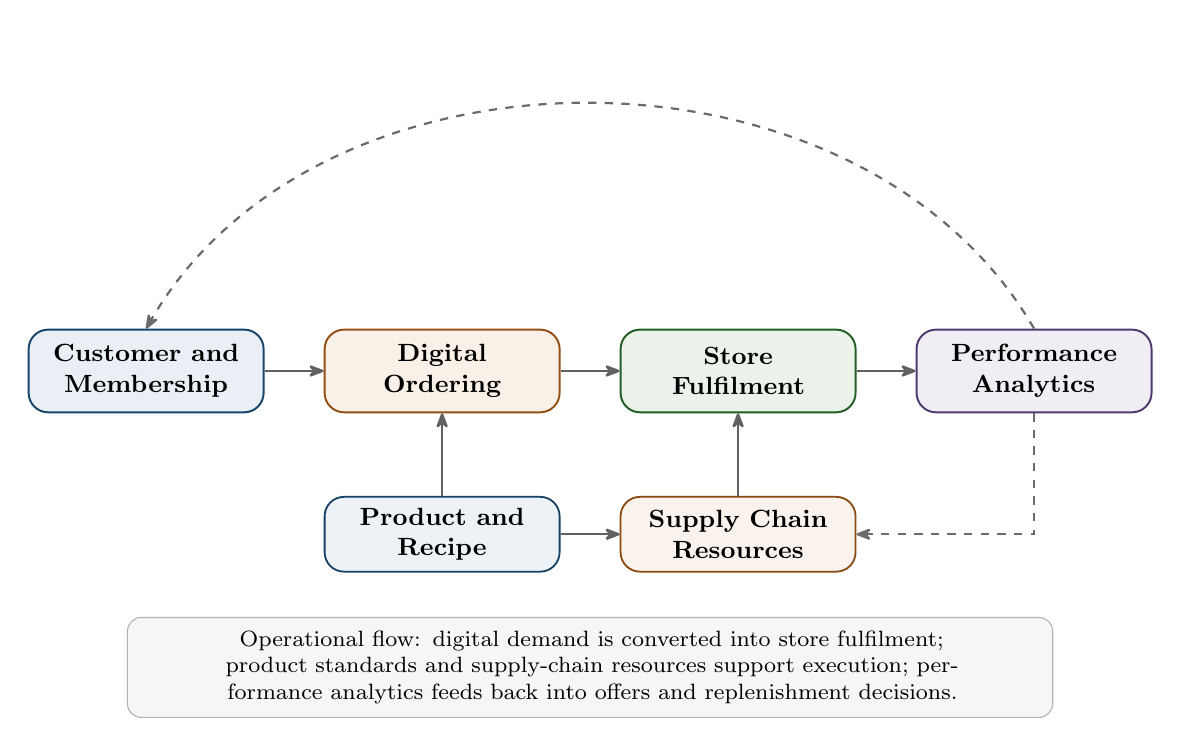
\begin{tikzpicture}[
    domain/.style={rectangle, rounded corners=7pt, draw=#1!75!black, fill=#1!10,
                   text width=2.75cm, minimum height=1.05cm, align=center,
                   font=\small\bfseries, line width=0.7pt},
    support/.style={rectangle, rounded corners=7pt, draw=#1!70!black, fill=#1!8,
                    text width=2.75cm, minimum height=0.95cm, align=center,
                    font=\small\bfseries, line width=0.65pt},
    arrow/.style={-{Stealth[round]}, line width=0.85pt, black!62},
    feedbackarrow/.style={-{Stealth[round]}, line width=0.8pt, dashed, black!58},
    note/.style={rectangle, rounded corners=5pt, draw=black!30, fill=lkgray,
                 text width=11.4cm, align=center, font=\footnotesize, inner sep=5pt}
  ]
    \node[domain=lkblue] (customer) {Customer and\\Membership};
    \node[domain=lkorange, right=0.75cm of customer] (order) {Digital\\Ordering};
    \node[domain=lkgreen, right=0.75cm of order] (store) {Store\\Fulfilment};
    \node[domain=lkpurple, right=0.75cm of store] (analytics) {Performance\\Analytics};

    \node[support=lkblue, below=1.05cm of order] (product) {Product and\\Recipe};
    \node[support=lkorange, below=1.05cm of store] (supply) {Supply Chain\\Resources};

    \draw[arrow] (customer) -- (order);
    \draw[arrow] (order) -- (store);
    \draw[arrow] (store) -- (analytics);
    \draw[arrow] (product) -- (order);
    \draw[arrow] (product) -- (supply);
    \draw[arrow] (supply) -- (store);
    \draw[feedbackarrow] (analytics.south) |- (supply.east);
    \draw[feedbackarrow] (analytics.north) to[out=120,in=60] (customer.north);

    \node[note, below=1.05cm of $(product)!0.5!(supply)$] {Operational flow: digital demand is converted into store fulfilment; product standards and supply-chain resources support execution; performance analytics feeds back into offers and replenishment decisions.};
  \end{tikzpicture}
  \caption{Scope of the conceptual model for Luckin Coffee.}
\end{figure}

The diagram uses business object boxes rather than database tables, so it remains readable for both business and technical stakeholders. The diagram presents the core objects and relationship IDs, while the following object table lists representative class variables, sum variables, count variables, and attributes in the notation used by the Seminar 4 examples. The relationships can later be translated into database entities, process models, or system architecture components.

% =================== NOTATION ===================
\section{Notation Used in the Conceptual Model}

The model follows the spirit of the examples in the Seminar 4 instruction sheet. Business objects are represented as boxes, and colours separate demand, fulfilment, resource, and analytics objects. Arrows indicate reading direction, while the relationship tables specify one-to-one, one-to-many, and many-to-many multiplicities.

\begin{table}[H]
\centering
\caption{Notation used in the conceptual model.}
\begin{tabularx}{\textwidth}{P{4.2cm}Y}
\toprule
\textbf{Notation} & \textbf{Meaning in this report} \\
\midrule
\textcolor{lkblue}{Class variables} & Variables used to classify an object, such as customer segment, store type, order channel, payment method, or product category. \\
\textcolor{lkorange}{Sum variables} & Quantitative values that can be summarised, such as order amount, discount amount, material cost, preparation time, or delivery fee. \\
\textcolor{lkgreen}{Count variables} & Numbers of objects or events, such as order count, item count, complaint count, stockout count, or visit count. \\
Additional attributes & Descriptive properties needed to identify or manage the object, such as customer ID, store ID, product name, recipe version, or supplier name. \\
Relationship arrows & Reading direction for the business relationship. For example, ``Customer places Order'' and ``Order is prepared by Store''. \\
Multiplicity & 1:N means one object can connect to many objects; M:N means many objects can connect to many objects; 1:1 means each object connects to one counterpart. \\
\bottomrule
\end{tabularx}
\end{table}

% =================== MAIN CONCEPTUAL MODEL ===================
\section{Conceptual Model for Luckin Coffee}

\begin{landscape}
\thispagestyle{empty}
\begin{figure}[H]
\portraitlandscapepagenumber
\centering
\footnotesize
\resizebox{0.965\linewidth}{!}{%
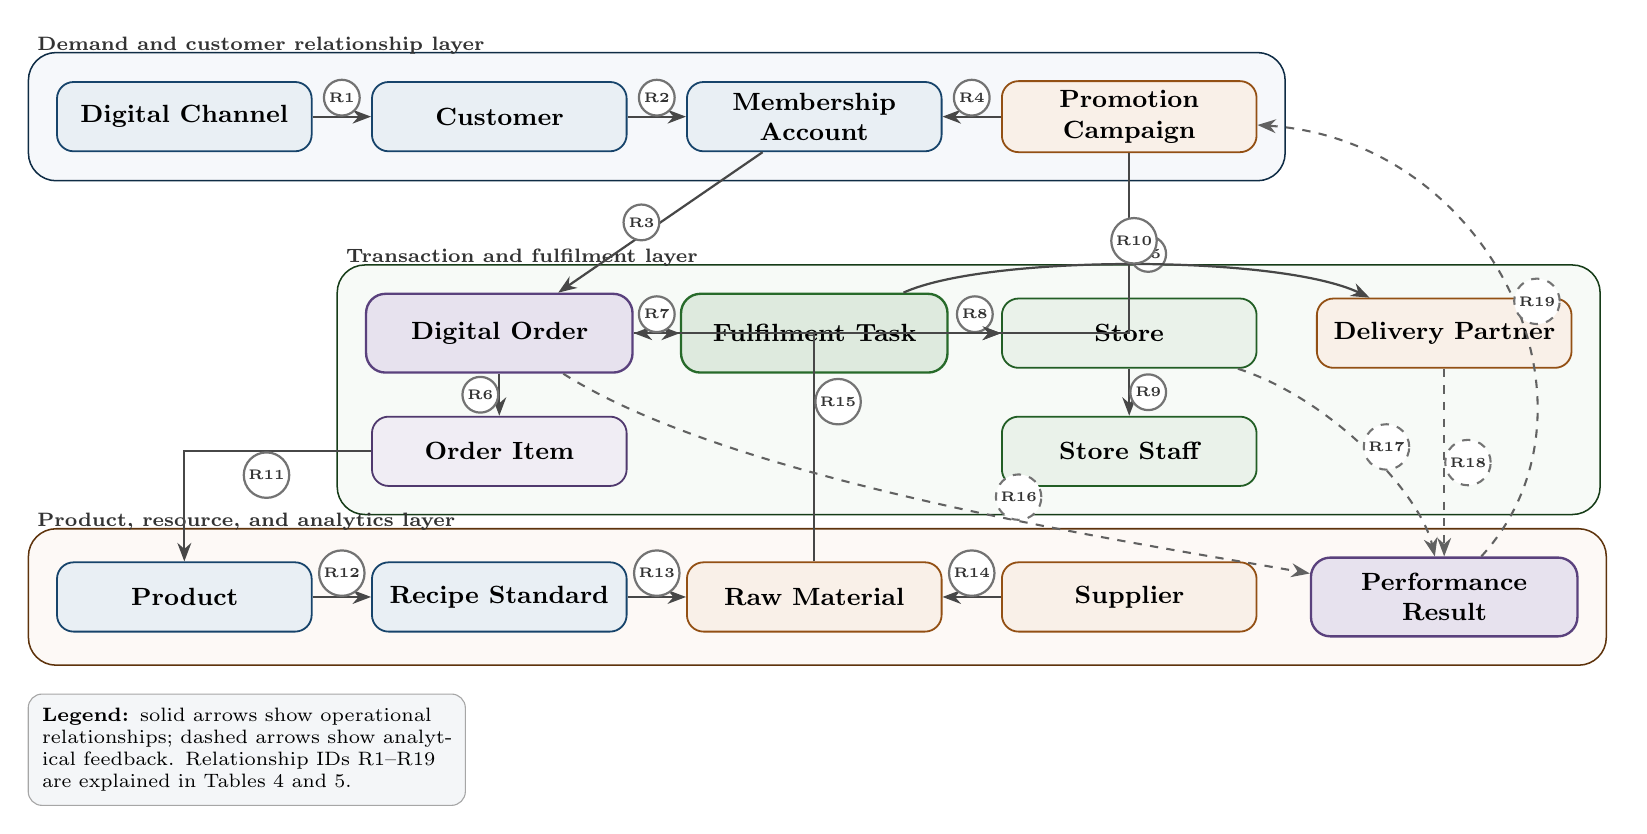
\begin{tikzpicture}[
  obj/.style={rectangle, rounded corners=6pt, draw=#1!75!black, fill=#1!10,
              text width=3.0cm, minimum height=0.88cm, align=center,
              font=\small\bfseries, line width=0.65pt},
  core/.style={rectangle, rounded corners=7pt, draw=#1!85!black, fill=#1!16,
               text width=3.15cm, minimum height=1.0cm, align=center,
               font=\small\bfseries, line width=0.85pt},
  group/.style={rectangle, rounded corners=10pt, draw=#1!48!black, fill=#1!4,
                inner sep=10pt, line width=0.55pt},
  rel/.style={-{Stealth[length=2.35mm]}, line width=0.8pt, black!72},
  feedback/.style={-{Stealth[length=2.35mm]}, line width=0.75pt, dashed, black!62},
  rtag/.style={circle, draw=black!55, fill=white, inner sep=1.15pt,
               font=\tiny\bfseries, text=darkgray},
  layerlabel/.style={font=\scriptsize\bfseries, text=darkgray},
  note/.style={rectangle, rounded corners=5pt, draw=black!35, fill=lkgray,
               text width=5.2cm, align=left, inner sep=5pt, font=\scriptsize}
]

% Customer and demand objects
\node[obj=lkblue] (channel) at (0,7.0) {Digital Channel};
\node[obj=lkblue] (customer) at (4.0,7.0) {Customer};
\node[obj=lkblue] (membership) at (8.0,7.0) {Membership Account};
\node[obj=lkorange] (promotion) at (12.0,7.0) {Promotion Campaign};

% Transaction and fulfilment objects
\node[core=lkpurple] (order) at (4.0,4.25) {Digital Order};
\node[obj=lkpurple] (orderitem) at (4.0,2.75) {Order Item};
\node[core=lkgreen] (task) at (8.0,4.25) {Fulfilment Task};
\node[obj=lkgreen] (store) at (12.0,4.25) {Store};
\node[obj=lkgreen] (staff) at (12.0,2.75) {Store Staff};
\node[obj=lkorange] (delivery) at (16.0,4.25) {Delivery Partner};

% Product, supply, and analytical objects
\node[obj=lkblue] (product) at (0,0.9) {Product};
\node[obj=lkblue] (recipe) at (4.0,0.9) {Recipe Standard};
\node[obj=lkorange] (material) at (8.0,0.9) {Raw Material};
\node[obj=lkorange] (supplier) at (12.0,0.9) {Supplier};
\node[core=lkpurple] (performance) at (16.0,0.9) {Performance Result};

% Background groups
\begin{scope}[on background layer]
  \node[group=lkblue, fit=(channel)(customer)(membership)(promotion)] (g1) {};
  \node[group=lkgreen, fit=(order)(orderitem)(task)(store)(staff)(delivery)] (g2) {};
  \node[group=lkorange, fit=(product)(recipe)(material)(supplier)(performance)] (g3) {};
\end{scope}

\node[layerlabel, above=0.08cm of g1.north west, anchor=west] {Demand and customer relationship layer};
\node[layerlabel, above=0.08cm of g2.north west, anchor=west] {Transaction and fulfilment layer};
\node[layerlabel, above=0.08cm of g3.north west, anchor=west] {Product, resource, and analytics layer};

% Main operational relationships
\draw[rel] (channel) -- node[rtag, midway, above] {R1} (customer);
\draw[rel] (customer) -- node[rtag, midway, above] {R2} (membership);
\draw[rel] (membership) -- node[rtag, midway, left] {R3} (order);
\draw[rel] (promotion) -- node[rtag, midway, above] {R4} (membership);
\draw[rel] (promotion) |- node[rtag, pos=0.28, right] {R5} (order);

\draw[rel] (order) -- node[rtag, midway, left] {R6} (orderitem);
\draw[rel] (order) -- node[rtag, midway, above] {R7} (task);
\draw[rel] (task) -- node[rtag, midway, above] {R8} (store);
\draw[rel] (store) -- node[rtag, midway, right] {R9} (staff);
\draw[rel] (task) .. controls (10.2,5.25) and (13.9,5.25) .. node[rtag, midway, above] {R10} (delivery);

\draw[rel] (orderitem) -| node[rtag, pos=0.28, below] {R11} (product);
\draw[rel] (product) -- node[rtag, midway, above] {R12} (recipe);
\draw[rel] (recipe) -- node[rtag, midway, above] {R13} (material);
\draw[rel] (supplier) -- node[rtag, midway, above] {R14} (material);
\draw[rel] (material) |- node[rtag, pos=0.35, right] {R15} (store);

% Analytical feedback relationships
\draw[feedback] (order) .. controls (7.0,2.35) and (12.0,1.6) .. node[rtag, pos=0.60, above] {R16} (performance);
\draw[feedback] (store) .. controls (14.6,3.4) and (15.7,2.2) .. node[rtag, pos=0.48, right] {R17} (performance);
\draw[feedback] (delivery) -- node[rtag, midway, right] {R18} (performance);
\draw[feedback] (performance) .. controls (18.2,3.3) and (16.6,6.7) .. node[rtag, pos=0.48, right] {R19} (promotion);

% Legend
\node[note, below=0.35cm of g3.south west, anchor=north west] {\textbf{Legend:} solid arrows show operational relationships; dashed arrows show analytical feedback. Relationship IDs R1--R19 are explained in Tables 4 and 5.};

\end{tikzpicture}%
}
\caption{Conceptual model of Luckin Coffee's mobile-first retail operating system. The diagram separates demand, fulfilment, resource, and analytics objects so that the main relationships remain readable; representative variables are listed in Table 3, and relationship meanings are explained in Tables 4 and 5.}
\end{figure}
\end{landscape}

The diagram shows Luckin Coffee as an integrated retail platform rather than a simple chain of coffee shops. The central object is the \textbf{Digital Order}. It connects customers, membership accounts, promotions, order items, fulfilment tasks, stores, and delivery partners. Around this core, products and recipes define what can be sold, suppliers and materials define what can be prepared, and performance results provide management feedback.

\begin{table}[H]
\centering
\scriptsize
\renewcommand{\arraystretch}{1.16}
\caption{Representative variables in the conceptual model.}
\begin{tabularx}{\textwidth}{P{3.0cm}Y Y Y Y}
\toprule
\textbf{Object} & \textbf{Class variables} & \textbf{Sum variables} & \textbf{Count variables} & \textbf{Attributes} \\
\midrule
Customer / Membership & Segment, city, age band, member tier & Points balance, coupon value & Visit count, order count & Customer ID, account ID \\
Digital Channel & Channel type, access device & Payment amount, discount value & Session count, redemption count & Channel ID, app version \\
Promotion Campaign & Campaign type, target segment & Budget, subsidy amount & Exposure count, redemption count & Campaign ID, valid period \\
Digital Order / Order Item & Order channel, payment method, product category & Order amount, item price, delivery fee & Item count, order count & Order ID, order time, status \\
Product / Recipe Standard & Category, season, launch region, quality grade & Standard cost, material dosage & Recipe version count & Product ID, recipe version \\
Store / Store Staff & Ownership type, city tier, staff role & Revenue, rent, labour cost, working hours & Order count, staff count & Store ID, staff ID \\
Raw Material / Supplier & Material type, origin, supplier type & Purchase cost, inventory value, contract amount & Batch count, delivery count, stockout count & Material ID, supplier ID \\
Fulfilment / Delivery / Performance & Task type, queue status, partner type, KPI type & Preparation time, waiting time, delivery fee, margin & Retry count, complaint count, delivery count & Task ID, partner ID, period \\
\bottomrule
\end{tabularx}
\end{table}

% =================== OBJECT EXPLANATION ===================
\section{Explanation of Main Objects}

\subsection{Customer, Membership Account, and Digital Channel}

The \textbf{Customer} object identifies the consumer and is classified by segment, city, and age band to explain demand differences across office workers, students, commuters, and other groups. A customer normally owns one \textbf{Membership Account}, which records digital identity, coupons, points, and order history. This reflects Luckin's dependence on digital membership rather than purely face-to-face customer management.

The \textbf{Digital Channel} object covers the mobile app, WeChat mini-program, e-commerce interfaces, and other access points. These channels capture visits, browsing, coupon redemption, and payment behaviour, making them both transaction interfaces and sources of demand data.

\subsection{Promotion Campaign and Digital Order}

The \textbf{Promotion Campaign} object covers coupons, membership discounts, new-product campaigns, seasonal offers, and targeted push messages. It is linked to both membership accounts and digital orders because one campaign can target many members and influence many purchases.

The \textbf{Digital Order} object is the operational centre of the model. It records channel, payment method, status, order time, order amount, discount amount, delivery fee, and item count. Separating orders from \textbf{Fulfilment Tasks} distinguishes the purchase event from the work required to complete it, such as preparation, pickup, delivery, or exception handling.

\subsection{Order Item, Product, and Recipe Standard}

The \textbf{Order Item} object decomposes a digital order into product lines, allowing item-level analysis of quantity, customisation, discount, popularity, and price sensitivity.

The \textbf{Product} object covers beverages, light food, packaged coffee, and merchandise. Its category, season, and launch region help describe Luckin's frequent product testing. The \textbf{Recipe Standard} object defines the operational rule behind each product, including recipe version, quality grade, dosage, standard cost, and SOP requirements. This separation expresses the difference between what the customer buys and how the store prepares it.

\subsection{Store, Store Staff, Raw Material, and Supplier}

The \textbf{Store} object covers self-operated and partnership stores, classified by ownership type, city tier, and location. Its revenue, rent, labour cost, order count, and staff count connect digital demand with local operating capacity.

The \textbf{Store Staff} object covers employees and managers who prepare orders and follow SOPs. Role, training status, working hours, productivity, and training modules are included because service consistency depends on both digital systems and human execution.

The \textbf{Raw Material} object covers coffee beans, milk, syrups, packaging, and other inputs, while the \textbf{Supplier} object identifies the external source of those materials. Together, they express the resource side of Luckin's model through origin, material type, batch status, purchase cost, inventory value, supplier certification, lead time, and delivery count.

\subsection{Fulfilment Task, Delivery Partner, and Performance Result}

The \textbf{Fulfilment Task} object records the operational work created by an order, including drink preparation, pickup handling, delivery handover, and exception processing. Task type, queue status, preparation time, waiting time, and retry count make store bottlenecks visible.

The \textbf{Delivery Partner} object covers external or platform-based logistics partners. Partner type, service area, delivery time, service fee, and delivery count are separated from store variables because delivery performance is partly outside direct store control but still affects customer experience.

The \textbf{Performance Result} object summarises operating outcomes by KPI type, period, region, revenue, margin, NPS score, complaint count, stockout count, and dashboard owner. It links orders, stores, promotions, and delivery outcomes to management evaluation.

% =================== RELATIONSHIP ANALYSIS ===================
\section{Relationship Analysis}

The main relationships in the model can be grouped into three layers. The first layer is the demand layer: customers use digital channels, maintain membership accounts, receive promotions, and place digital orders. The second layer is the fulfilment layer: orders contain order items, order items refer to products, products are prepared according to recipe standards, and fulfilment tasks are executed by stores and delivery partners. The third layer is the control layer: stores, orders, promotions, stock conditions, and delivery outcomes are summarised into performance results.

\begin{table}[H]
\centering
\small
\renewcommand{\arraystretch}{1.18}
\caption{Demand, order, and fulfilment relationships in the conceptual model.}
\begin{tabularx}{\textwidth}{P{1.0cm}P{4.0cm}P{1.5cm}Y}
\toprule
\textbf{ID} & \textbf{Relationship} & \textbf{Type} & \textbf{Business meaning and measures enabled} \\
\midrule
R1 & Digital Channel -- Customer & 1:N & Channels such as the app and mini-program capture customer visits, sessions, and campaign exposure. \\
R2 & Customer -- Membership Account & 1:1 & Customer identity is connected with points, coupons, and order history; this supports active-member and repeat-purchase analysis. \\
R3 & Membership Account -- Digital Order & 1:N & One member may place many orders across time, stores, and channels; this enables order-frequency, AOV, and customer-lifetime-value analysis. \\
R4 & Promotion Campaign -- Membership Account & M:N & Campaigns target many members, while members may receive many campaigns; this supports targeting and redemption analysis. \\
R5 & Promotion Campaign -- Digital Order & M:N & Campaigns influence orders, and one order may use more than one promotional mechanism; this enables subsidy and conversion-rate tracking. \\
R6 & Digital Order -- Order Item & 1:N & Order-level payment and fulfilment status are separated from product-level quantity, customisation, and item discount information. \\
R7 & Digital Order -- Fulfilment Task & 1:N & A customer order can create preparation, pickup, delivery, or exception-handling tasks; this supports preparation-time and completion-rate monitoring. \\
R8 & Fulfilment Task -- Store & N:1 & Many fulfilment tasks are prepared by one store, making store capacity, labour utilisation, and queue delay measurable. \\
R9 & Store -- Store Staff & 1:N & Stores employ staff whose training status and productivity affect service consistency and operating efficiency. \\
R10 & Fulfilment Task -- Delivery Partner & N:1 & Delivery tasks are assigned to logistics partners, allowing delivery time, delivery fee, and completion rate to be evaluated. \\
\bottomrule
\end{tabularx}
\end{table}

\begin{table}[H]
\centering
\small
\renewcommand{\arraystretch}{1.18}
\caption{Product, resource, and analytical feedback relationships in the conceptual model.}
\begin{tabularx}{\textwidth}{P{1.0cm}P{4.0cm}P{1.5cm}Y}
\toprule
\textbf{ID} & \textbf{Relationship} & \textbf{Type} & \textbf{Business meaning and measures enabled} \\
\midrule
R11 & Order Item -- Product & N:1 & Many order lines can refer to the same product; this enables product sales, gross margin, and new-product success analysis. \\
R12 & Product -- Recipe Standard & 1:N & A product may have recipe versions across time or regions, supporting controlled innovation and operational standardisation. \\
R13 & Recipe Standard -- Raw Material & M:N & Recipes consume multiple materials and materials may support multiple recipes; this supports ingredient-use, cost-ratio, and wastage analysis. \\
R14 & Supplier -- Raw Material & 1:N & Suppliers provide material batches or categories for store replenishment; this enables lead-time, delivery-count, and quality-pass-rate evaluation. \\
R15 & Raw Material -- Store & M:N & Stores consume and hold materials from multiple batches, supporting inventory turnover, stockout, and replenishment analysis. \\
R16 & Digital Order -- Performance Result & 1:N & Orders feed analytical results such as revenue, discount amount, order value, and transaction success rate. \\
R17 & Store -- Performance Result & 1:N & Store operations generate periodic financial and service KPIs, including daily revenue, margin, complaints, and stockouts. \\
R18 & Delivery Partner -- Performance Result & 1:N & Delivery partners generate service KPIs such as delivery completion time, delivery success rate, and logistics cost per order. \\
R19 & Performance Result -- Promotion Campaign & 1:N & Analytical feedback improves future promotion design by showing which campaigns produce durable loyalty rather than only short-term discount purchases. \\
\bottomrule
\end{tabularx}
\end{table}

This relationship structure supports both operational analysis and future database design. For example, if management wants to know why delivery complaints increased in a city, the model suggests which objects should be connected: customer complaints can be traced to digital orders, fulfilment tasks, delivery partners, stores, and time periods. If management wants to evaluate a new product, the model connects order items, product categories, recipe standards, raw material consumption, promotion campaigns, and performance results.

% =================== BUSINESS SCENARIOS ===================
\section{Business Scenarios Supported by the Model}

\subsection{Scenario 1: Mobile Order and Store Pickup}

A customer opens the app or WeChat mini-program, receives a personalised coupon, selects a drink, pays digitally, and chooses pickup. The model traces this process from customer and membership account to promotion campaign, digital order, order item, fulfilment task, store preparation, pickup, feedback, and KPI update.

\begin{figure}[H]
  \centering
  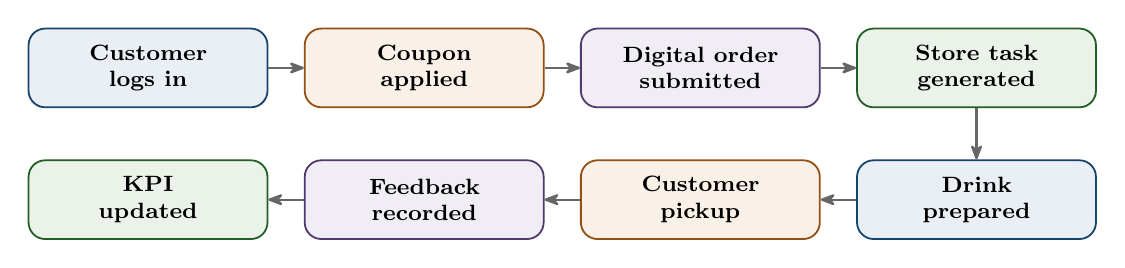
\begin{tikzpicture}[
    step/.style={rectangle, rounded corners=6pt, draw=#1!75!black, fill=#1!10,
                 text width=2.8cm, minimum height=1.0cm, align=center,
                 font=\footnotesize\bfseries, line width=0.65pt},
    arrow/.style={-{Stealth[round]}, line width=0.8pt, black!60}
  ]
    \node[step=lkblue] (s1) {Customer\\logs in};
    \node[step=lkorange, right=0.45cm of s1] (s2) {Coupon\\applied};
    \node[step=lkpurple, right=0.45cm of s2] (s3) {Digital order\\submitted};
    \node[step=lkgreen, right=0.45cm of s3] (s4) {Store task\\generated};
    \node[step=lkblue, below=0.65cm of s4] (s5) {Drink\\prepared};
    \node[step=lkorange, left=0.45cm of s5] (s6) {Customer\\pickup};
    \node[step=lkpurple, left=0.45cm of s6] (s7) {Feedback\\recorded};
    \node[step=lkgreen, left=0.45cm of s7] (s8) {KPI\\updated};

    \draw[arrow] (s1) -- (s2);
    \draw[arrow] (s2) -- (s3);
    \draw[arrow] (s3) -- (s4);
    \draw[arrow] (s4) -- (s5);
    \draw[arrow] (s5) -- (s6);
    \draw[arrow] (s6) -- (s7);
    \draw[arrow] (s7) -- (s8);
  \end{tikzpicture}
  \caption{Pickup-order scenario supported by the conceptual model.}
\end{figure}

\subsection{Scenario 2: New Product Launch and Performance Review}

Luckin frequently launches new drinks and evaluates them through sales data. In the model, a new product receives a product record and recipe standard, appears in digital channels, may be supported by a campaign, and is then measured through order-item data, raw-material use, margin, complaints, and supply stability.

\subsection{Scenario 3: Store Capacity and Delivery Reliability}

During peak demand, the model captures pressure through digital orders and fulfilment tasks. If preparation time, waiting time, or delivery completion deteriorates, management can compare staff scheduling, material availability, delivery partner capacity, and store-level order volume.

% =================== FROM CONCEPTUAL MODEL TO DATABASE ===================
\section{Implications for Future Database Design}

Although this report is conceptual rather than technical, the model provides a foundation for database design. Each object can become a candidate entity or table, and each relationship can become a foreign-key relationship, bridge table, or transaction link. For example, the many-to-many relationship between recipe standards and raw materials would require a recipe-material bridge, while the one-to-many relationship between digital orders and order items would normally become separate order and order-line tables.

\begin{table}[H]
\centering
\caption{How the conceptual model can guide future database design.}
\begin{tabularx}{\textwidth}{P{4.1cm}Y}
\toprule
\textbf{Conceptual modelling decision} & \textbf{Database design implication} \\
\midrule
Separate customer from membership account & Customer demographic and segment information can be managed separately from app account, points, coupon, and authentication-related data. \\
Separate digital order from order item & Order-level payment and fulfilment status can be stored independently from product-level quantity, customisation, and item discount data. \\
Separate product from recipe standard & Product catalogue information can remain stable while recipe versions and SOP rules change over time. \\
Represent recipe-material as M:N & A bridge table would be needed to record material dosage, standard cost, and recipe version for each ingredient. \\
Separate fulfilment task from digital order & Operational execution can be analysed even when one order creates multiple tasks, such as preparation and delivery handover. \\
Include performance result as an analytical object & KPI reporting can aggregate operational data by store, period, region, product, campaign, and delivery partner. \\
\bottomrule
\end{tabularx}
\end{table}

The model also prevents premature database design mistakes. If the system stored only orders and products, it would be difficult to analyse fulfilment delay, recipe compliance, supply-chain pressure, or campaign effectiveness. Including fulfilment tasks, recipe standards, raw materials, suppliers, promotions, and performance results preserves the business meaning needed for later enterprise architecture and database work.

% =================== CONCLUSION ===================
\section{Conclusion}

This report created a conceptual model for Luckin Coffee as a technology-driven new retail coffee enterprise. The model identifies the main objects---customer, membership account, digital channel, promotion campaign, digital order, order item, product, recipe standard, raw material, supplier, store, store staff, fulfilment task, delivery partner, and performance result---and explains how they support customer ordering, product preparation, store fulfilment, supply-chain replenishment, delivery coordination, and KPI feedback.

The model connects Luckin's strategic logic with operational reality. Customer value is created through the coordination of digital demand capture, physical fulfilment, recipe standardisation, supply support, and performance measurement. The model is therefore detailed enough to support later database design while remaining conceptual enough to clarify the business structure before technical implementation.

\begingroup
\small
\setlength{\itemsep}{0pt}
\begin{thebibliography}{9}

\bibitem{luckin2025results}
Luckin Coffee Inc. (2026).
\emph{Luckin Coffee Announces Fourth Quarter and Fiscal Year 2025 Financial Results}.
\href{https://investor.luckincoffee.com/news-releases/news-release-details/luckin-coffee-announces-fourth-quarter-and-fiscal-year-2025/}{Luckin Coffee Investor Relations}.

\bibitem{luckin2025annual}
Luckin Coffee Inc. (2026).
\emph{Form 20-F Annual Report for the Fiscal Year Ended December 31, 2025}.
\href{https://www.sec.gov/Archives/edgar/data/1767582/000110465926035712/lk-20251231x20f.htm}{U.S. Securities and Exchange Commission}.

\bibitem{kaplan1992bsc}
Kaplan, R. S., \& Norton, D. P. (1992).
\emph{The Balanced Scorecard: Measures That Drive Performance}.
Harvard Business Review, 70(1), 71--79.

\bibitem{osterwalder2010bmg}
Osterwalder, A., \& Pigneur, Y. (2010).
\emph{Business Model Generation: A Handbook for Visionaries, Game Changers, and Challengers}.
John Wiley \& Sons.

\end{thebibliography}
\endgroup

\end{document}
